\documentclass[11pt,a4paper]{report}
\usepackage[textwidth=37em,vmargin=30mm]{geometry}
\usepackage{calc,xunicode,amsmath,amssymb,paralist,enumitem,tabu,booktabs,datetime2,xeCJK,xeCJKfntef,listings}
\usepackage{tocloft,fancyhdr,tcolorbox,xcolor,graphicx,eso-pic,xltxtra,xelatexemoji}

\newcommand{\envyear}[0]{2025}
\newcommand{\envdatestr}[0]{2025-02-16}
\newcommand{\envfinaldir}[0]{webdb/2025/20250216/final}

\usepackage[hidelinks]{hyperref}
\hypersetup{
    colorlinks=false,
    pdfpagemode=FullScreen,
    pdftitle={Web Digest - \envdatestr}
}

\setlength{\cftbeforechapskip}{10pt}
\renewcommand{\cftchapfont}{\rmfamily\bfseries\large\raggedright}
\setlength{\cftbeforesecskip}{2pt}
\renewcommand{\cftsecfont}{\sffamily\small\raggedright}

\setdefaultleftmargin{2em}{2em}{1em}{1em}{1em}{1em}

\usepackage{xeCJK,xeCJKfntef}
\xeCJKsetup{PunctStyle=plain,RubberPunctSkip=false,CJKglue=\strut\hskip 0pt plus 0.1em minus 0.05em,CJKecglue=\strut\hskip 0.22em plus 0.2em}
\XeTeXlinebreaklocale "zh"
\XeTeXlinebreakskip = 0pt


\setmainfont{Brygada 1918}
\setromanfont{Brygada 1918}
\setsansfont{IBM Plex Sans}
\setmonofont{JetBrains Mono NL}
\setCJKmainfont{Noto Serif CJK SC}
\setCJKromanfont{Noto Serif CJK SC}
\setCJKsansfont{Noto Sans CJK SC}
\setCJKmonofont{Noto Sans CJK SC}

\setlength{\parindent}{0pt}
\setlength{\parskip}{8pt}
\linespread{1.15}

\lstset{
	basicstyle=\ttfamily\footnotesize,
	numbersep=5pt,
	backgroundcolor=\color{black!5},
	showspaces=false,
	showstringspaces=false,
	showtabs=false,
	tabsize=2,
	captionpos=b,
	breaklines=true,
	breakatwhitespace=true,
	breakautoindent=true,
	linewidth=\textwidth
}






\newcommand{\coverpic}[2]{
    % argv: itemurl, authorname
    Cover photo by #2~~(\href{#1}{#1})
}
\newcommand{\makeheader}[0]{
    \begin{titlepage}
        % \newgeometry{hmargin=15mm,tmargin=21mm,bmargin=12mm}
        \begin{center}
            
            \rmfamily\scshape
            \fontspec{BaskervilleF}
            \fontspec{Old Standard}
            \fontsize{59pt}{70pt}\selectfont
            WEB\hfill DIGEST
            
            \vfill
            % \vskip 30pt
            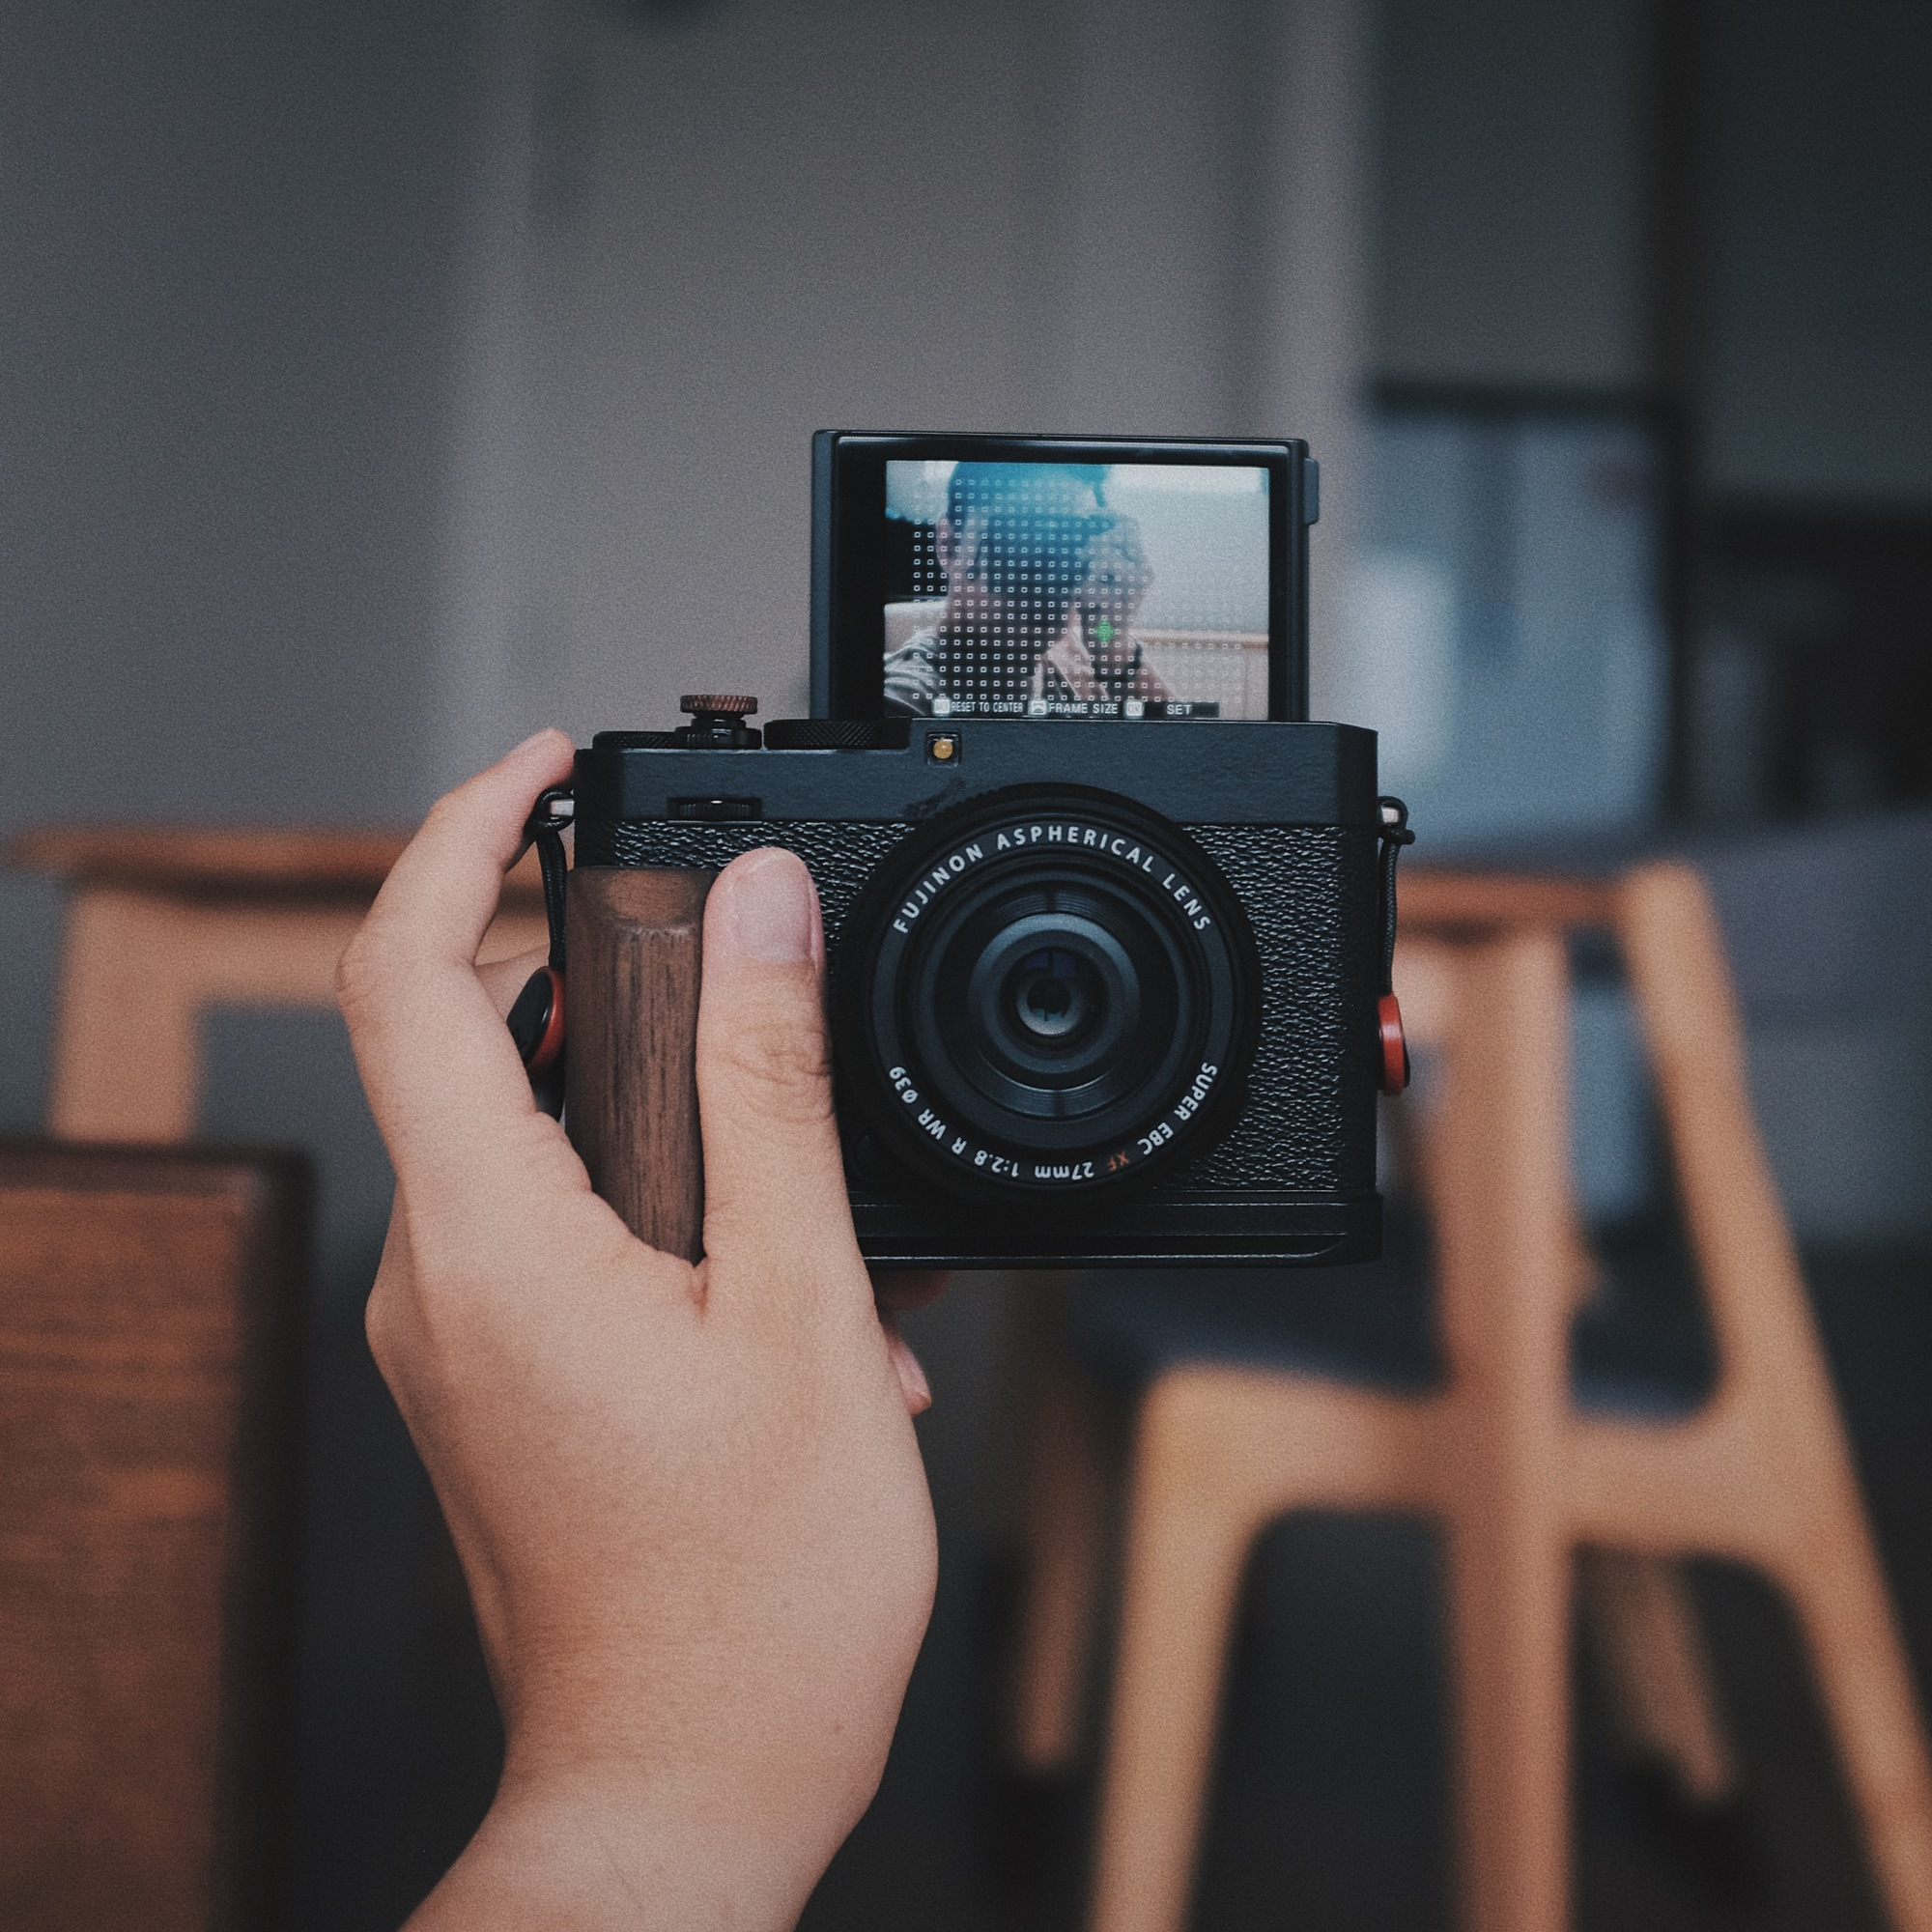
\includegraphics[width=\linewidth]{\envfinaldir/coverpic-prod.jpg}\par
            % \vskip 30pt
            \vfill

            \normalsize\rmfamily\scshape
            \copyright{} The Web Digest Project \hfill\large \envdatestr
        \end{center}
    \end{titlepage}
    % \restoregeometry
}
\newcommand{\simplehref}[1]{%
    \textcolor{blue!80!green}{\href{#1}{#1}}%
}
\renewcommand{\contentsname}{\center\Huge\sffamily\bfseries Contents\par\vskip 20pt}
\newcounter{ipartcounter}
\setcounter{ipartcounter}{0}
\newcommand{\ipart}[1]{
    % \vskip 20pt
    \clearpage
    \stepcounter{ipartcounter}
    \phantomsection
    \addcontentsline{toc}{chapter}{#1}
    % \begin{center}
    %     \Huge
    %     \sffamily\bfseries
    %     #1
    % \end{center}
    % \vskip 20pt plus 7pt
}
\newcounter{ichaptercounter}
\setcounter{ichaptercounter}{0}
\newcommand{\ichapter}[1]{
    % \vskip 20pt
    \clearpage
    \stepcounter{ichaptercounter}
    \phantomsection
    \addcontentsline{toc}{section}{\numberline{\arabic{ichaptercounter}}#1}
    \begin{center}
        \Huge
        \sffamily\bfseries
        #1
    \end{center}
    \vskip 20pt plus 7pt
}
\newcommand{\entrytitlefont}[1]{\subsection*{\raggedright\Large\sffamily\bfseries#1}}
\newcommand{\entryitemGeneric}[2]{
    % argv: title, url
    \parbox{\linewidth}{
        \entrytitlefont{#1}\par\vskip 5pt
        \footnotesize\ttfamily\mdseries
        \simplehref{#2}
    }\vskip 11pt plus 11pt minus 1pt
}
\newcommand{\entryitemGithub}[3]{
    % argv: title, url, desc
    \parbox{\linewidth}{
        \entrytitlefont{#1}\par\vskip 5pt
        \footnotesize\ttfamily\mdseries
        \simplehref{#2}\par\vskip 5pt
        \small\rmfamily\mdseries#3
    }\vskip 11pt plus 11pt minus 1pt
}
\newcommand{\entryitemAp}[3]{
    % argv: title, url, desc
    \parbox{\linewidth}{
        \entrytitlefont{#1}\par\vskip 5pt
        \footnotesize\ttfamily\mdseries
        \simplehref{#2}\par\vskip 5pt
        \small\rmfamily\mdseries#3
    }\vskip 11pt plus 11pt minus 1pt
}
\newcommand{\entryitemHackernews}[3]{
    % argv: title, hnurl, rawurl
    % \parbox{\linewidth}{
    %     \entrytitlefont{#1}\par\vskip 5pt
    %     \footnotesize\ttfamily\mdseries
    %     \simplehref{#3}\par
    %     \textcolor{black!50}{\href{#2}{#2}}
    % }\vskip 11pt plus 11pt minus 1pt
    \begin{minipage}{\linewidth}
            \entrytitlefont{#1}\par\vskip 5pt
            \footnotesize\ttfamily\mdseries
            \simplehref{#3}\par
            \textcolor{black!50}{\href{#2}{#2}}
    \end{minipage}\par\vskip 11pt plus 11pt minus 1pt
}







\begin{document}

\makeheader

\tableofcontents\clearpage




\ipart{Developers}
\ichapter{Hacker News}
\entryitemTwoLinks{The European VAT Is Not a Discriminatory Tax Against US Exports}{https://news.ycombinator.com/item?id=43062457}{https://taxfoundation.org/blog/trump-reciprocal-tariffs-eu-vat-discriminatory/}

\entryitemTwoLinks{My Life in Weeks}{https://news.ycombinator.com/item?id=43061498}{https://weeks.ginatrapani.org/}

\entryitemTwoLinks{New SF public health chief was part of McKinsey opioid-marketing operation}{https://news.ycombinator.com/item?id=43061482}{https://sfstandard.com/2025/02/14/san-francisco-department-public-health-daniel-tsai-opioids-mckinsey/}

\entryitemTwoLinks{Alzheimer's biomarkers now visible up to a decade ahead of symptoms}{https://news.ycombinator.com/item?id=43060587}{https://newatlas.com/brain/alzheimers-dementia/alzheimers-biomarkers-visible-decade-before-symptoms/}

\entryitemTwoLinks{Deepseek R1 Distill 8B Q40 on 4 x Raspberry Pi 5}{https://news.ycombinator.com/item?id=43059579}{https://github.com/b4rtaz/distributed-llama/discussions/162}

\entryitemTwoLinks{Carbon capture more costly than switching to renewables, researchers find}{https://news.ycombinator.com/item?id=43058997}{https://techxplore.com/news/2025-02-carbon-capture-renewables.html}

\entryitemTwoLinks{Dust from car brakes more harmful than exhaust, study finds}{https://news.ycombinator.com/item?id=43058993}{https://e360.yale.edu/digest/brake-pads-lung-damage-study}

\entryitemTwoLinks{Amazon's killing a feature that let you download and backup Kindle books}{https://news.ycombinator.com/item?id=43058889}{https://www.theverge.com/news/612898/amazon-removing-kindle-book-download-transfer-usb}

\entryitemTwoLinks{Diablo hackers uncovered a speedrun scandal}{https://news.ycombinator.com/item?id=43058522}{https://arstechnica.com/gaming/2025/02/the-diablo-hackers-that-debunked-a-record-speedrun/}

\entryitemTwoLinks{Twelve months at 1.5 °C signals earlier than expected breach of Paris Agreement}{https://news.ycombinator.com/item?id=43058311}{https://www.nature.com/articles/s41558-025-02247-8}

\entryitemTwoLinks{The Impact of Generative AI on Critical Thinking [pdf]}{https://news.ycombinator.com/item?id=43057907}{https://www.microsoft.com/en-us/research/uploads/prod/2025/01/lee\_2025\_ai\_critical\_thinking\_survey.pdf}

\entryitemTwoLinks{Show HN: Kreuzberg – Modern async Python library for document text extraction}{https://news.ycombinator.com/item?id=43057375}{https://github.com/Goldziher/kreuzberg}

\entryitemTwoLinks{Jane Street's Figgie card game}{https://news.ycombinator.com/item?id=43057344}{https://www.figgie.com/}

\entryitemTwoLinks{If you believe in "Artificial Intelligence", take five minutes to ask it}{https://news.ycombinator.com/item?id=43056831}{https://svpow.com/2025/02/14/if-you-believe-in-artificial-intelligence-take-five-minutes-to-ask-it-about-stuff-you-know-well/}

\entryitemTwoLinks{Bookshop.org launches Kindle alternative, sends e-book sales to local bookstores}{https://news.ycombinator.com/item?id=43056526}{https://www.usatoday.com/story/entertainment/books/2025/01/28/bookshop-org-ereader-ebook-app/77928209007/}

\entryitemTwoLinks{The 20 year old PSP can now connect to WPA2 WiFi Networks}{https://news.ycombinator.com/item?id=43055671}{https://wololo.net/2025/02/14/the-20-year-old-psp-can-now-connect-to-wpa2-wifi-networks/}

\entryitemTwoLinks{Q2DOS – Quake 2 backported to MS-DOS}{https://news.ycombinator.com/item?id=43054963}{https://dk.toastednet.org/Q2DOS/}

\entryitemTwoLinks{Men claiming to be from DOGE show up at San Francisco City Hall, demand records}{https://news.ycombinator.com/item?id=43054892}{https://www.cbsnews.com/sanfrancisco/news/doge-3-men-show-up-at-sf-city-hall-demand-records/}

\entryitemTwoLinks{Did Semgrep Just Get a Lot More Interesting?}{https://news.ycombinator.com/item?id=43054673}{https://fly.io/blog/semgrep-but-for-real-now/}

\entryitemTwoLinks{Wyden Releases Draft Bill to Secure Americans' Communications}{https://news.ycombinator.com/item?id=43054632}{https://www.wyden.senate.gov/news/press-releases/wyden-releases-draft-bill-to-secure-americans-communications-against-foreign-surveillance-demands}\ichapter{Phoronix}
\entryitemGeneric{\hskip 0pt{}NTSYNC Driver Fix Being Worked On For Proper User Permissions}{https://www.phoronix.com/news/Linux-NTSYNC-Permissions-Issue}

\entryitemGeneric{\hskip 0pt{}Karol Herbst Steps Down As Nouveau Maintainer Due To Linux Kernel's Toxic Environment}{https://www.phoronix.com/news/Karol-Herbst-Nouveau-No}

\entryitemGeneric{\hskip 0pt{}KDE Developers Addressing Early Bugs From Plasma 6.3}{https://www.phoronix.com/news/KDE-Plasma-6.3-Early-Bugs}

\entryitemGeneric{\hskip 0pt{}Ikey Doherty's Serpent OS Rebranding As AerynOS}{https://www.phoronix.com/news/Serpent-OS-To-AerynOS}

\entryitemGeneric{\hskip 0pt{}Go 1.24 Brings Performance Improvements, Better WebAssembly Support}{https://www.phoronix.com/news/Go-1.24-Released}

\entryitemGeneric{\hskip 0pt{}Dynamic Triple Buffering Merged For GNOME 48}{https://www.phoronix.com/news/GNOME-48-Triple-Buffering}

\entryitemGeneric{\hskip 0pt{}Linux 6.15 To Ensure PlayStation 5 Controllers Use The Correct Driver}{https://www.phoronix.com/news/Linux-6.15-Ensures-PS5-Driver}

\entryitemGeneric{\hskip 0pt{}Fwupd 2.0.6 Adds Support For HPE Gen10/Gen10+ Servers}{https://www.phoronix.com/news/Fwupd-2.0.6-Released}

\entryitemGeneric{\hskip 0pt{}Ubuntu Making Progress On Replacing initramfs-tools With Dracut}{https://www.phoronix.com/news/Ubuntu-Dracut-Still-WIP}\ichapter{Dribbble}
\entryitemGeneric{\hskip 0pt{}Alpaca}{https://dribbble.com/shots/25627851-Alpaca}

\entryitemGeneric{\hskip 0pt{}Ethereum Wordmark Logo Concept}{https://dribbble.com/shots/25623390-Ethereum-Wordmark-Logo-Concept}

\entryitemGeneric{\hskip 0pt{}Illustration}{https://dribbble.com/shots/25619766-Illustration}

\entryitemGeneric{\hskip 0pt{}Carbon Solutions B2B Dashboard Design}{https://dribbble.com/shots/25554521-Carbon-Solutions-B2B-Dashboard-Design}

\entryitemGeneric{\hskip 0pt{}Love Potion}{https://dribbble.com/shots/25619714-Love-Potion}

\entryitemGeneric{\hskip 0pt{}Pirate Parrot}{https://dribbble.com/shots/25619077-Pirate-Parrot}

\entryitemGeneric{\hskip 0pt{}Mortar\&Carrot}{https://dribbble.com/shots/25619708-Mortar-Carrot}

\entryitemGeneric{\hskip 0pt{}SPROXX - LOGO DESIGN}{https://dribbble.com/shots/25619328-SPROXX-LOGO-DESIGN}

\entryitemGeneric{\hskip 0pt{}Master / God / Cloud}{https://dribbble.com/shots/25619810-Master-God-Cloud}

\entryitemGeneric{\hskip 0pt{}Fast Turn Fittings}{https://dribbble.com/shots/25619395-Fast-Turn-Fittings}

\entryitemGeneric{\hskip 0pt{}Sidebar Quick Actions: Integrations}{https://dribbble.com/shots/25618236-Sidebar-Quick-Actions-Integrations}

\entryitemGeneric{\hskip 0pt{}Black Cat Speed Shop®}{https://dribbble.com/shots/25614666-Black-Cat-Speed-Shop}

\entryitemGeneric{\hskip 0pt{}Fintech icons pack download}{https://dribbble.com/shots/25607159-Fintech-icons-pack-download}

\entryitemGeneric{\hskip 0pt{}Self Love}{https://dribbble.com/shots/25607914-Self-Love}

\entryitemGeneric{\hskip 0pt{}Urban Echo}{https://dribbble.com/shots/25608526-Urban-Echo}

\entryitemGeneric{\hskip 0pt{}Cloaked Wireless Device}{https://dribbble.com/shots/25403560-Cloaked-Wireless-Device}

\entryitemGeneric{\hskip 0pt{}Logo tip 001. Symmetry and asymmetry}{https://dribbble.com/shots/25606111-Logo-tip-001-Symmetry-and-asymmetry}

\entryitemGeneric{\hskip 0pt{}Sentinal - Logo Design}{https://dribbble.com/shots/25606497-Sentinal-Logo-Design}

\entryitemGeneric{\hskip 0pt{}World Peace}{https://dribbble.com/shots/25609765-World-Peace}

\entryitemGeneric{\hskip 0pt{}Tanuki}{https://dribbble.com/shots/25606258-Tanuki}

\entryitemGeneric{\hskip 0pt{}Dirty Dutch - Brand Mark / Logo}{https://dribbble.com/shots/25604523-Dirty-Dutch-Brand-Mark-Logo}

\entryitemGeneric{\hskip 0pt{}Cast AI Logo Redesign}{https://dribbble.com/shots/25607135-Cast-AI-Logo-Redesign}

\entryitemGeneric{\hskip 0pt{}Running Partners}{https://dribbble.com/shots/25606250-Running-Partners}

\entryitemGeneric{\hskip 0pt{}Android Dynamic Island}{https://dribbble.com/shots/25604942-Android-Dynamic-Island}


\ipart{Developers~~~~(zh-Hans)}
\ichapter{Solidot}
\entryitemGeneric{\hskip 0pt{}亚马逊将关闭 Kindle 的 Download \& Transfer via USB 功能}{https://www.solidot.org/story?sid=80564}

\entryitemGeneric{\hskip 0pt{}摩根大通 CEO 对反对重返办公室的意见不屑一顾}{https://www.solidot.org/story?sid=80563}

\entryitemGeneric{\hskip 0pt{}20 光年外的一颗恒星宜居带有行星}{https://www.solidot.org/story?sid=80562}

\entryitemGeneric{\hskip 0pt{}美摄起诉字节跳动抄袭代码获赔 8266.8 万元}{https://www.solidot.org/story?sid=80561}

\entryitemGeneric{\hskip 0pt{}俄罗斯无人机攻击切尔诺贝利核电站}{https://www.solidot.org/story?sid=80560}

\entryitemGeneric{\hskip 0pt{}Zed 使用开源模型 Zeta 预测用户的编辑}{https://www.solidot.org/story?sid=80559}

\entryitemGeneric{\hskip 0pt{}Arm 将自己制造芯片}{https://www.solidot.org/story?sid=80558}

\entryitemGeneric{\hskip 0pt{}作为换囚交易的一部分美国释放了 BTC-e 联合创始人}{https://www.solidot.org/story?sid=80557}

\entryitemGeneric{\hskip 0pt{}攻读博士学位的人数在减少}{https://www.solidot.org/story?sid=80556}

\entryitemGeneric{\hskip 0pt{}中国居民对 AI 的信任高于美国}{https://www.solidot.org/story?sid=80555}

\entryitemGeneric{\hskip 0pt{}研究发现 AI 的新闻摘要会经常性的扭曲事实}{https://www.solidot.org/story?sid=80554}

\entryitemGeneric{\hskip 0pt{}Google 和苹果恢复上架 TikTok}{https://www.solidot.org/story?sid=80553}

\entryitemGeneric{\hskip 0pt{}Google 计划用机器学习估计用户的年龄}{https://www.solidot.org/story?sid=80552}

\entryitemGeneric{\hskip 0pt{}印度儿童的心算能力不能转变学校里的数学分数}{https://www.solidot.org/story?sid=80551}

\entryitemGeneric{\hskip 0pt{}百度宣布文心一言 4 月 1 日起免费}{https://www.solidot.org/story?sid=80550}

\entryitemGeneric{\hskip 0pt{}丰田等多家日企内部禁用 DeepSeek}{https://www.solidot.org/story?sid=80549}

\entryitemGeneric{\hskip 0pt{}科学家探测到迄今最高能的中微子}{https://www.solidot.org/story?sid=80548}

\entryitemGeneric{\hskip 0pt{}大脑中的微塑料是否会伤害你?}{https://www.solidot.org/story?sid=80547}

\entryitemGeneric{\hskip 0pt{}NOAA 公开泰坦号内爆音频}{https://www.solidot.org/story?sid=80546}

\entryitemGeneric{\hskip 0pt{}汤森路透在美国赢得 AI 版权侵犯诉讼}{https://www.solidot.org/story?sid=80545}\ichapter{V2EX}
\entryitemGeneric{\hskip 0pt{}[Android] Google pixel 手机质量真是堪忧}{https://www.v2ex.com/t/1111718}

\entryitemGeneric{\hskip 0pt{}[问与答] 究竟什么样的大模型服务值得付费订阅。购买和搭建?}{https://www.v2ex.com/t/1111717}

\entryitemGeneric{\hskip 0pt{}[Python] 有人在生产环境用 Sanic 吗?有什么需要注意的坑吗?看起来性能很强还轻量。我记得以前这个框架有乱关闭长连接的 Bug,花了一年多才修复}{https://www.v2ex.com/t/1111716}

\entryitemGeneric{\hskip 0pt{}[问与答] 导师评价网为何难以建立,是有什么不好规避的法规问题吗?补充}{https://www.v2ex.com/t/1111715}

\entryitemGeneric{\hskip 0pt{}[信息安全] 为什么 iOS 有很多能越狱的漏洞, Android 却比较少有能在不解锁 BL 的情况下 ROOT 的洞?只是因为没人愿意挖吗?}{https://www.v2ex.com/t/1111714}

\entryitemGeneric{\hskip 0pt{}[问与答] 导师评价网为何难以建立,是有什么不好规避的法规问题吗?}{https://www.v2ex.com/t/1111713}

\entryitemGeneric{\hskip 0pt{}[宽带症候群] 我这边的家宽开始阻断 hy 协议了。}{https://www.v2ex.com/t/1111712}

\entryitemGeneric{\hskip 0pt{}[Windows] 有好兄弟知道电脑 spdif 接口不能输出 5.1 声道是什么情况吗}{https://www.v2ex.com/t/1111711}

\entryitemGeneric{\hskip 0pt{}[程序员] 8 卡 H100 部署 DeepSeekR1 求助}{https://www.v2ex.com/t/1111710}

\entryitemGeneric{\hskip 0pt{}[程序员] 之前一直在终端设备上做去广告, 最近部署了 Adguard Home 发现是真好用啊, 大伙还在自己的 NAS/服务器上部署了什么有用或者有趣的东西吗?}{https://www.v2ex.com/t/1111709}

\entryitemGeneric{\hskip 0pt{}[程序员] 关于 docker 的一些问题?}{https://www.v2ex.com/t/1111708}

\entryitemGeneric{\hskip 0pt{}[职场话题] 代写专利交底书,顺便出售几篇写好的}{https://www.v2ex.com/t/1111707}

\entryitemGeneric{\hskip 0pt{}[分享发现] 分享新买的设备 -- 懒猫微服}{https://www.v2ex.com/t/1111706}

\entryitemGeneric{\hskip 0pt{}[电影] 有没有治愈电影或者电视推荐}{https://www.v2ex.com/t/1111705}

\entryitemGeneric{\hskip 0pt{}[程序员] 有没有做股票量化的朋友}{https://www.v2ex.com/t/1111704}

\entryitemGeneric{\hskip 0pt{}[Java] 我公开了我的项目,有大佬可以帮忙解决无效的绑定问题吗?}{https://www.v2ex.com/t/1111703}

\entryitemGeneric{\hskip 0pt{}[问与答] 请问有没有分析软件代码库的 AI 应用}{https://www.v2ex.com/t/1111702}

\entryitemGeneric{\hskip 0pt{}[NAS] 4 盘位的 NAS(TS-464C),使用哪两个盘位来组 RAID1 比较合适?}{https://www.v2ex.com/t/1111701}

\entryitemGeneric{\hskip 0pt{}[分享创造] 原研药查询小程序:原研汇 v1.1 更新计划}{https://www.v2ex.com/t/1111700}

\entryitemGeneric{\hskip 0pt{}[耳机] 求推荐有线的开放式耳机。}{https://www.v2ex.com/t/1111699}

\entryitemGeneric{\hskip 0pt{}[程序员] taro 好像烂尾了}{https://www.v2ex.com/t/1111696}

\entryitemGeneric{\hskip 0pt{}[分享创造] 分享一个基于大语言模型驱动的多轮评审的高质量英文文章翻译方案}{https://www.v2ex.com/t/1111695}

\entryitemGeneric{\hskip 0pt{}[分享创造] 随机食物小程序}{https://www.v2ex.com/t/1111693}

\entryitemGeneric{\hskip 0pt{}[分享发现] bybitCard 最近挺火的,但请注意}{https://www.v2ex.com/t/1111691}

\entryitemGeneric{\hskip 0pt{}[投资] XIRR 计算年化收益率为负,但总收益金额为正,该如何理解?}{https://www.v2ex.com/t/1111690}

\entryitemGeneric{\hskip 0pt{}[分享发现] 小米公司创立 15 年了}{https://www.v2ex.com/t/1111688}

\entryitemGeneric{\hskip 0pt{}[问与答] 请教下各位看日剧有哪些渠道?}{https://www.v2ex.com/t/1111687}

\entryitemGeneric{\hskip 0pt{}[程序员] Cursor 编辑器,如何删除 chat 和 composer 的记录?}{https://www.v2ex.com/t/1111686}

\entryitemGeneric{\hskip 0pt{}[分享发现] 有没有人试过用 AI 来生成角色动画?我发现了一个有趣的工具}{https://www.v2ex.com/t/1111685}

\entryitemGeneric{\hskip 0pt{}[音乐] 你们心中可以封神的音乐有哪些?}{https://www.v2ex.com/t/1111684}

\entryitemGeneric{\hskip 0pt{}[广州] 广州 薪酬结构}{https://www.v2ex.com/t/1111683}

\entryitemGeneric{\hskip 0pt{}[问与答] 各位,求推荐好玩的体感游戏 APP}{https://www.v2ex.com/t/1111682}

\entryitemGeneric{\hskip 0pt{}[Apple] 求推荐 iOS 中的照片消除软件}{https://www.v2ex.com/t/1111681}

\entryitemGeneric{\hskip 0pt{}[分享创造] 用 Tauri 开发了一个跟 Raycast 长得一样的跨平台启动器}{https://www.v2ex.com/t/1111680}

\entryitemGeneric{\hskip 0pt{}[macOS] 求助一个很诡异的扩展坞问题}{https://www.v2ex.com/t/1111678}

\entryitemGeneric{\hskip 0pt{}[分享创造] 小工具,交互式魔方,在线玩魔方}{https://www.v2ex.com/t/1111677}

\entryitemGeneric{\hskip 0pt{}[随想] 一线城市大部分打工人最终的归属就是回老家吗}{https://www.v2ex.com/t/1111676}

\entryitemGeneric{\hskip 0pt{}[iOS] 求推荐 iOS 中的照片消除 App}{https://www.v2ex.com/t/1111674}

\entryitemGeneric{\hskip 0pt{}[问与答] 急,在线等,超过 10 天, win11 怎么退回 win10?}{https://www.v2ex.com/t/1111673}

\entryitemGeneric{\hskip 0pt{}[分享创造] [送码] Twitter 粉丝数量小组件 App}{https://www.v2ex.com/t/1111672}

\entryitemGeneric{\hskip 0pt{}[汽车] 买车的误区:以智能驾驶为第一买车需求}{https://www.v2ex.com/t/1111671}

\entryitemGeneric{\hskip 0pt{}[OpenAI] 今天突然发现 chatgpt 的对话无法编辑了,这是为什么}{https://www.v2ex.com/t/1111670}

\entryitemGeneric{\hskip 0pt{}[Apple] iPhone 能实现快速重启手机的快捷指令么?}{https://www.v2ex.com/t/1111669}

\entryitemGeneric{\hskip 0pt{}[问与答] 2025 年 PVE 软路由选 n100 还是 j4125 纠结中!}{https://www.v2ex.com/t/1111668}

\entryitemGeneric{\hskip 0pt{}[职场话题] 如果连续 4 周都没有工作内容,如何应对每天的站会?}{https://www.v2ex.com/t/1111667}

\entryitemGeneric{\hskip 0pt{}[汽车] 又来问车子了,第二辆车,买熊猫 MINI 和 五菱 MINI EV,哪一款好,有开过的介绍一下经验吗?}{https://www.v2ex.com/t/1111666}

\entryitemGeneric{\hskip 0pt{}[深圳] 宝安上川公寓转租}{https://www.v2ex.com/t/1111665}

\entryitemGeneric{\hskip 0pt{}[Apple] Mac 外接罗技 C1000E 摄像头好模糊}{https://www.v2ex.com/t/1111664}

\entryitemGeneric{\hskip 0pt{}[程序员] 有没有使用过 ai 外呼系统的老哥}{https://www.v2ex.com/t/1111663}

\entryitemGeneric{\hskip 0pt{}[职场话题] 咨询一下香港薪资和深圳薪资的换算比例}{https://www.v2ex.com/t/1111661}


\ipart{Generic News}







\clearpage
\leavevmode\vfill
\footnotesize

Copyright \copyright{} 2023-2025 Neruthes and other contributors.

This document is published with CC BY-NC-ND 4.0 license.

The entries listed in this newsletter may be copyrighted by their respective creators.

This newsletter is generated by the Web Digest project.

The newsletters are also delivered via Telegram channel \CJKunderline{\href{https://t.me/webdigestchannel}{https://t.me/webdigestchannel}}.\\
RSS feed is available at \CJKunderline{\href{https://webdigest.pages.dev/rss.xml}{https://webdigest.pages.dev/rss.xml}}.

This newsletter is available in PDF at
\CJKunderline{\href{https://webdigest.pages.dev/}{https://webdigest.pages.dev/}}.

The source code being used to generate this newsletter is available at\\
\CJKunderline{\href{https://github.com/neruthes/webdigest}{https://github.com/neruthes/webdigest}}.

This newsletter is also available in
\CJKunderline{\href{http://webdigest.pages.dev/readhtml/\envyear/WebDigest-20250216.html}{HTML}} and
\CJKunderline{\href{https://github.com/neruthes/webdigest/blob/master/markdown/\envyear/WebDigest-20250216.md}{Markdown}}.


\coverpic{https://unsplash.com/photos/a-person-standing-in-a-field-with-the-sun-in-the-background-vzJOgLWhU8I}{Rafael Garcin}


\end{document}
